\section{Basics}


\subsection{Default Surface Parameterization}

From the user point of view, the simplest entry point to this package
is the following function:

\ccFunction{Parameterizer_traits_3<ParameterizationMesh_3>::Error_code parameterize (ParameterizationMesh_3 & mesh);}
{
Compute a one-to-one mapping from a 3D triangle surface 'mesh' to a 2D circle, using Floater Mean Value Coordinates algorithm. A one-to-one mapping is guaranteed.
The mapping is piecewise linear on the input mesh triangles. The result is a (u,v) pair of parameter coordinates for each vertex of the input mesh.
Preconditions:\begin{itemize}
\item 'mesh' must be a surface with one connected component.\item 'mesh' must be a triangular mesh.\end{itemize}
}

The \ccc{CGAL::parameterize()} function applies a default surface parameterization
method: Floater Mean Value Coordinates~\cite{cgal:f-mvc-03}, with an
arc-length circular border parameterization, and using OpenNL sparse
linear solver~\cite{cgal:l-nmdgp-05}.

The \ccc{ParameterizationMesh_3} concept defines the input meshes handled
by \ccc{CGAL::parameterize()}. See Section \ref{sec:Input-Mesh-for-parameterize}.

The result is stored into the (u,v) fields of the mesh halfedges.

Note: \ccc{CGAL::Parameterizer_traits_3<ParameterizationMesh_3>} is the (pure virtual)
superclass of all surface parameterizations and defines the error codes.


\subsection{Input Mesh for parameterize()}
\label{sec:Input-Mesh-for-parameterize}

The general definition of input meshes handled by \ccc{CGAL::parameterize()} is:

\begin{itemize}

\item Triangulated.

\item 2-manifold.

\item Oriented.

\item Homeomorphic to a disc (may have holes).

\end{itemize}

These input meshes must be models of the \ccc{ParameterizationMesh_3} concept.
In fact, \ccc{ParameterizationMesh_3} is a general concept to access to a
polyhedral mesh.
It is optimized for the \ccc{Surface_mesh_parameterization} package
only in the sense that it
defines the accessors to fields specific to the parameterization domain
(\ccc{index}, \ccc{u}, \ccc{v}, \ccc{is_parameterized}).

The extra constraints  needed by the surface parameterization methods (triangulated,
2-manifold, homeomorphic to a disc) are not part of the concept and
are checked at runtime.

This package provides a model of the \ccc{ParameterizationMesh_3} concept
to access \ccc{CGAL::Polyhedron_3<Traits>}:

\ccc{CGAL::Parameterization_polyhedron_adaptor_3<Polyhedron_3_>}  \\


\subsection{Default Parameterization Example}

\ccc{Simple_parameterization.C} applies the default parameterization to a
\ccc{CGAL::Polyhedron_3<Traits>} mesh (must be a topological disk).
Eventually, it extracts the result from halfedges and prints it.

\ccIncludeExampleCode{Surface_mesh_parameterization/Simple_parameterization.C}


\subsection{Enhanced parameterize() function}

This package provides a second \ccc{CGAL::parameterize()} entry point
where the user can specify a parameterization method:

\ccFunction{Parameterizer_traits_3<ParameterizationMesh_3>::Error_code parameterize (ParameterizationMesh_3 & mesh, ParameterizerTraits_3 parameterizer);}
{
Compute a one-to-one mapping from a 3D triangle surface 'mesh' to a simple 2D domain. The mapping is piecewise linear on the triangle mesh. The result is a pair (u,v) of parameter coordinates for each vertex of the input mesh.
One-to-one mapping may be guaranteed or not, depending on the chosen \ccc{ParametizerTraits_3} algorithm.
Preconditions:\begin{itemize}
\item 'mesh' must be a surface with one connected component.\item 'mesh' must be a triangular mesh.\item the mesh border must be mapped onto a convex polygon (for fixed border parameterizations).\end{itemize}
}


\subsection{Introduction to the Package Concepts}

\subsubsection{The ParameterizerTraits\_3 concept}

This \cgal\ package implements some of the state-of-the-art
surface parameterization methods, such as Least Squares Conformal Maps,
Discrete Conformal Map, Discrete Authalic
Parameterization, Floater Mean Value Coordinates or Tutte Barycentric
Mapping. These methods are provided as models of the
\ccc{ParameterizerTraits_3} concept.
See Section \ref{sec:Surface-Parameterization-Methods}.

Each of these surface parameterization methods is templated by
the input mesh type, a border parameterization and a solver:

% Insert image parameterizer_class_diagram_simplified.png/eps
% with title "A parameterizer UML class diagram (simplified)"
\begin{center}
    \label{Surface_mesh_parameterization-fig-parameterizer_class_diagram_simplified}
    % Image
    \begin{ccTexOnly}
        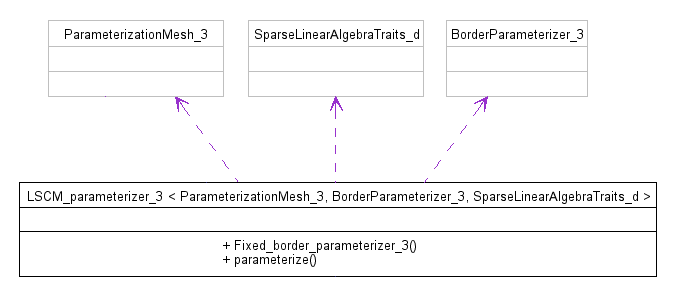
\includegraphics[width=0.80\textwidth]{Surface_mesh_parameterization/parameterizer_class_diagram_simplified} % omit .eps suffix
    \end{ccTexOnly}
    \begin{ccHtmlOnly}
        <img width="80%" border=0 src="./parameterizer_class_diagram_simplified.png"><P>
    \end{ccHtmlOnly}
    % Title
    \begin{figure}[h]
        \caption{A parameterizer UML class diagram (simplified)}
    \end{figure}
\end{center}


\subsubsection{The BorderParameterizer\_3 concept}

Parameterization methods for
borders are used as traits classes modifying the behavior of
\ccc{ParameterizerTraits_3} models.
They are provided as models of the \ccc{BorderParameterizer_3} concept.
See Sections \ref{sec:Border-Parameterizations-for-Fixed-Methods}
and \ref{sec:Border-Parameterizations-for-Free-Methods}.


\subsubsection{The SparseLinearAlgebraTraits\_d concept}

This package solves sparse linear systems using solvers which are models
of \ccc{SparseLinearAlgebraTraits_d}.
See Section \ref{sec:Sparse-Linear-Algebra}.


\subsubsection{The ParameterizationMesh\_3 and ParameterizationPatchableMesh\_3 Concepts}

We saw in Section \ref{sec:Input-Mesh-for-parameterize}
that the input meshes handled by \ccc{CGAL::parameterize()}
must be models of the \ccc{ParameterizationMesh_3} concept.

We also saw that the surface parameterization methods in this package only support
surfaces that are homeomorphic to disks. How about non disk-like meshes?

\emph{In practice}, the input mesh can be of any genus and
have any number of connected components. If it is not a topological
disc, it has to come with a description of a cutting path (an oriented list of
vertices) which is the border of a topological disc.  If no cutting path is
given as input, we assume that the surface border is the longest border already
in the input mesh (the other borders will be considered as holes).

For this purpose, the
\ccc{CGAL::Parameterization_mesh_patch_3<ParameterizationPatchableMesh_3>}
class is responsible for \emph{virtually} cutting
a patch in a \ccc{ParameterizationPatchableMesh_3} mesh.
The resulting patch is a topological
disk (if the input cutting path is correct)
and provides a \ccc{ParameterizationMesh_3} interface. It can be used as
parameter of \ccc{CGAL::parameterize()}.

\ccc{ParameterizationPatchableMesh_3} inherits from \ccc{ParameterizationMesh_3},
thus is a concept for a 3D surface mesh.
\ccc{ParameterizationPatchableMesh_3} adds the ability to support patches and
virtual seams. \emph{Patches} are a subset of a 3D mesh.
\emph{Virtual seams} are the ability
to behave exactly as if the surface was cut along a certain path.

See more information in Section \ref{sec:Cutting-a-Mesh}.
